\section{From A Posterior with Gaussian Distributions to an least-squares Objective-Function}
\label{appendix:PDtoL2}

In this appendix, we develop the operations necessary to go from a posterior distribution formulation to an objective function in the case of the Tikhonov inverse problem.

We stated in section \ref{section:keys} that a least-squares term corresponds to a Gaussian prior. For a vector of parameters, the multivariate Gaussian distribution, denoted by $\mathcal{N}$, with mean $\mathbf{\mu}$ and covariance $\Sigma$ (denoted by $\sigma^2$ for a unidimensional Gaussian, with $\sigma$ being the standard-deviation) is:

\begin{align}
&\mathcal{N}(\mathbf{m}|\mathbf{\mu}, \Sigma) = {\frac{\exp(-\frac{1}{2}||\Sigma^{-\frac{1}{2}}(\mathbf{m}-\mathbf{\mu})||_2^2)}{\sqrt{(2\pi)^n\det(\Sigma)}}} \label{GaussianDef_2}
\end{align}

Going from a posterior distribution to an objective function is done by taking the negative natural logarithm of the posterior. Taking the negative logarithm of a single Gaussian term gives:

\begin{align}
&-\log(\mathcal{N}(\mathbf{m}|\mathbf{\mu}, \Sigma)) = \frac{1}{2}||\Sigma^{-\frac{1}{2}}(\mathbf{m}-\mathbf{\mu})||_2^2 + \log({\sqrt{(2\pi)^n\det(\Sigma)}}) \label{LogGaussian}
\end{align}

The first term obtained in equation \ref{LogGaussian} is recognizable as a least-squares misfit. The second term does not depend on $\mathbf{m}$ and is thus a constant. As constants do not play any role in the optimization, it is thus discarded in the objective function.

For the full Tikhonov geophysical objective function $\mathcal{P}(\mathbf{m}|\mathbf{d}_{\text{obs}})$, the full posterior distributions can be written, using the Bayes rules, as:

\begin{align}
&\mathcal{P}(\mathbf{m}|\mathbf{d}_{\text{obs}}) = \frac{\mathcal{P}(\mathbf{d}_{\text{obs}}|\mathbf{m})\mathcal{P}(\mathbf{m})}{\mathcal{P}(\mathbf{d}_{\text{obs}})} \label{appendix:Bayes}\\
\end{align}
with: 
\begin{align}
&\mathcal{P}(\mathbf{d}_{\text{obs}}|\mathbf{m}) = \mathcal{N}(\mathcal{F}\lbrack\mathbf{m}\rbrack|\mathbf{d}_{\text{obs}}, (W_d^TW_d)^{-1}) \\
\end{align}
\begin{align}
&\mathcal{P}(\mathbf{m}) = \mathcal{N}(\mathbf{m}|\mathbf{m}_{{\text{ref}}}, (\beta\alpha_sW_s^TW_s)^{-1})\mathcal{N}(\mathbf{m}|\mathbf{m}_{{\text{ref}}},(\beta L^TL)^{-1})
\end{align}

where the finite difference operator $L$ summarizes the first or second derivatives in all directions with their respective $\{\alpha\}$ scale. We respectively express the data misfit, the smallness and smoothness probability functions as Gaussian distributions:

\begin{align}
&\mathcal{N}(\mathbf{d}_{\text{obs}}|\mathbf{m}, (W_d^TW_d)^{-1}) = {\frac{\exp(-\frac{1}{2}||W_d(\mathcal{F}\lbrack\mathbf{m}\rbrack-\mathbf{d}_{\text{obs}})||_2^2)}{\sqrt{(2\pi)^n\det(\lbrack W_d^TW_d\rbrack^{-1})}}} \label{DataMisfitGaussian}\\
\end{align}
\begin{align}
&\mathcal{N}(\mathbf{m}|\mathbf{m}_{{\text{ref}}}, (\beta\alpha_sW_s^TW_s)^{-1}) = {\frac{\exp(-\frac{1}{2}||W_s(\mathbf{m}-\mathbf{m}_{{\text{ref}}})||_2^2)^{\beta\alpha_s}}{\sqrt{(2\pi)^n\det(\lbrack \beta\alpha_sW_s^TW_s\rbrack^{-1})}}} \label{SmallnessGaussian}\\
\end{align}
\begin{align}
&\mathcal{N}(\mathbf{m}|\mathbf{m}_{{\text{ref}}}, (\beta L^TL)^{-1}) = {\frac{\exp(-\frac{1}{2}||L_i(\mathbf{m}-\mathbf{m}_{{\text{ref}}})||_2^2)^{\beta}}{\sqrt{(2\pi)^n\det(\lbrack \beta L^TL\rbrack^{-1})}}} \label{SmoothnessGaussian}
\end{align}

The objective function is obtained by applying the negative natural logarithm to the posterior distribution described in equation \ref{appendix:Bayes}. The summation form is simply a consequence of the fundamental property of the logarithm function, the multiplication becomes an addition in this new space. It follows:

\begin{align}
\Phi(\mathbf{m}) &= \frac{1}{2}||W_d(\mathcal{F}\lbrack\mathbf{m}\rbrack-\mathbf{d}_{\text{obs}})||_2^2 + \frac{\beta\alpha_s}{2}||W_s(\mathbf{m}-\mathbf{m}_{{\text{ref}}})||_2^2 + \nonumber\\  &~\frac{\beta}{2}||L(\mathbf{m}-\mathbf{m}_{{\text{ref}}})||_2^2 +\text{Constant} \label{fullObjFct}
\end{align}

The constant term in equation \ref{fullObjFct} contains the constant terms for each Gaussian distribution and the constant term $log(\mathcal{P}(\mathbf{d}_{\text{obs}}))$.

This completes the detailed operation to go from a posterior distribution to an objective function formulation of the Tikhonov inverse problem.


%%%%%%%%%%%%%%%%%%%%%%%%%%%%%%%%%%%%%%%%%%%%%%%%%%%%%%%%%%%%%%%%%%%%%%%%%%%%%%%
\appendix{conjugate prior versus semi-conjugate prior for means and variances prior information for a single univariate Gaussian Distribution} \label{Appendix:full_conjugate}

\begin{figure*}
    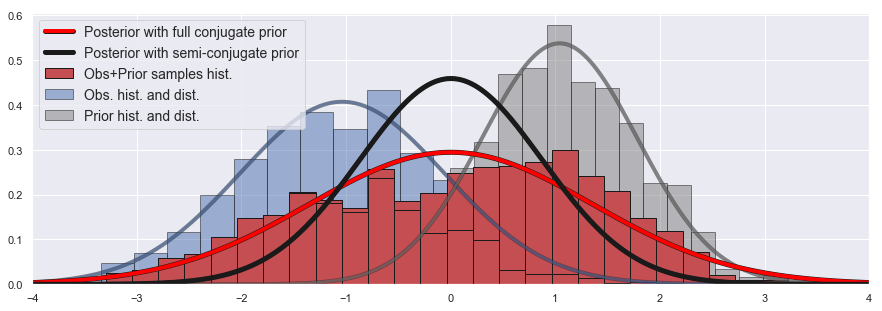
\includegraphics[width=\textwidth]{./Fig/LowRes/Full_vs_Semi_conjugate.png}
    \caption{A comparison of the MLE estimations of the mean and variance for a single one dimensional Gaussian distribution (no prior), semi-conjugate prior and full conjugate prior MAPs. We have observed samples in blue, along with their estimated MLE Gaussian distribution, and a prior distribution in gray. Using confidence values of unity in the prior is similar to having an equal number of samples from the prior and in the observed data sets. A synthetic prior sample set is represented as the gray histogram. The posterior distribution with a semi-conjugate prior is in black and is seen as an average of the parameters of the observed and prior distributions. The posterior distribution with a full conjugate prior is in red. The red histogram is obtained by merging the observed samples with the synthetic prior samples. This histogram corresponds to the posterior distribution with a full conjugate prior. Note that the variance is larger than for either of the two original distributions; this results because of  the difference in the means. Legend: Hist. stands for histogram; Dist. stands for distribution; Obs. stands for observed samples.}
    \label{Full_vs_Semi_conjugate}
\end{figure*}

In this section, we elaborate on the difference between a full and a semi-conjugate prior approach for estimating the parameters of a single, one dimensional, Gaussian distribution. After giving the needed definitions for the full conjugate prior and how the MAP-EM updates are affected, we illustrate the difference between semi and full conjugate through the example displayed in Fig. \ref{Full_vs_Semi_conjugate}.

We first need some definitions. The full conjugate prior for the mean and variance follows a Normal-Inverse-Gamma distribution \citep{Murphy:2012:MLP:2380985}. As in section \ref{UpdateTheta}, we use the Normal-Inverse Chi-Squared re-parameterization:

\begin{align}
&\mathcal{P}({\mu},\sigma^2) = \mathcal{N}\mathcal{X}^{-2}({\mu}, \sigma^2|{\mu}_{prior}, K, N,\sigma_{prior}^2) \label{mu_sigma_prior}
\end{align}
With the confidences $K$ in the prior mean and $N$ in the prior variance:
\begin{align}
&{K}=({\kappa}{\pi}_{prior}V)^{-1}\\
&{N}={\nu}{\pi}_{prior}V
\end{align}

The update of the means in MAP-EM algorithm stays the same as for the semi-conjugate prior approach, as detailed in equation \ref{mu_update}. On the contrary the update of the variances now requires an additional term ${s_{\bar{{\mu}}}}_j^{(k)}$ to account for the difference between the observed and the prior means:

\begin{align}
&{\sigma_j^2}^{(k)} = \frac{{{V_{j}^{(k)}} {\sigma^2_{\bar{\mathbf{m}}}}_j}^{(k)} + \nu_j {\pi_j}_{prior} V {\sigma_j^2}_{prior}+ {s_{\bar{{\mu}}}}_j^{(k)} }
{{V_{j}^{(k)}} + \nu_j {\pi_j}_{prior} V} \label{sig_update_full}\\
\end{align}
with:
\begin{align}
&{\sigma^2_{\bar{\mathbf{m}}}}_j^{(k)} =\frac{1}{{V_{j}^{(k)}}} \sum_{i=1}^{n} v_i n_{ij}^{(k)}({m}_i-\bar{{m}_j}^{(k)})^2\\
\end{align}
\begin{align}
&{s_{\bar{{\mu}}}}_j^{(k)} = \frac{\kappa_j V_{j}^{(k)} }{\kappa_j + V_{j}^{(k)}}(\bar{{m}}_j^{(k)}-{{\mu}_{j}}_{prior})^2 \label{full_additionalterm}
\end{align}

We illustrate those concepts with Fig. \ref{Full_vs_Semi_conjugate}. Let us consider the following setup. We have a set of observations (in our framework, this was our geophysical model), represented through their histogram in blue. The Gaussian distribution in blue represents the MLE parameters (estimated without any prior information). We now add prior information in the form of a Gaussian distribution, in gray in the Fig. \ref{Full_vs_Semi_conjugate}. We set the confidence parameters $\kappa$ and $\nu$ to unity, meaning that we have equal confidence in the observations and the prior ($\zeta$ is irrelevant here as we have only one Gaussian distribution). This equal confidence can be represented by having an equal number of samples from the prior than in the observed set. The histogram of this prior synthetic samples set set is shown in gray.

The full conjugate prior approach can be understood as fitting a Gaussian distribution on the dataset formed by merging the observed and synthetic observations; this is represented in Fig. \ref{Full_vs_Semi_conjugate} in red. The full conjugate MAP distribution, also in red, is well centered between the two observed and prior distribution as expected, and so is the semi-conjugate distribution (in black). However the variance of the red histogram, and thus of the posterior distribution with full conjugate prior, is higher than the variance of either the observed or prior distribution. This is due to the difference in the means of the two distributions, which the full conjugate prior approach accounts for (see equations \ref{sig_update_full} and \ref{full_additionalterm}). The semi-conjugate prior approach considers the means and variances independently (see equations \ref{mu_semiprior} and \ref{sigma_semiprior}). The MAP mean estimates are the same for both priors.

The semi-conjugate prior approach seems a better choice in the context of geophysical inversion. As our goal with this framework is to differentiate various geological units, by guiding the geophysical model to reproduce certain features, the full conjugate prior approach is sometimes detrimental as it can drive the variance further from the prior than what is currently seen in the model at each iteration.


%%%%%%%%%%%%%%%%%%%%%%%%%%%%%%%%%%%%%%%%%%%%%%%%%%%%%%%%%%%%%%%%%%%%%%%%%%%%%%%
\section{Pseudocode algorithm} \label{section:pseudocode}

\begin{algorithm}[ht!]
    %\setstretch{1}
    \SetKwInOut{Initialization}{Initialization}
    \caption{This algorithm finds a geophysical model reproducing the geophysical, petrophysical and geological data.}
    \label{algo:algorithm}
    \nl \Initialization{
    \begin{itemize}
    \item \underline{Input:}
    \begin{itemize}
        \item Initial geophysical model $\mathbf{m}^{(0)}$, petrophysical distributions $\Theta^{(0)}$ and geological model $\mathbf{z}^{(0)}$.
    \end{itemize}

    \item \underline{Parameters:}
    \begin{itemize}
      \item \textit{Objective function}: data's noise matrix $W_d$, trade-off parameter $\beta^{(0)}$, prior matrices and weights $\left\{\alpha\right\}$, ${\left\{W\right\}}$.
      \item \textit{Localized prior}: specific $\mathcal{P}(z_i)$ for available locations $i \in \{1..n\}$, local weights $\left\{\mathbf{w}_{i}\right\}_{i=1..n}$.
      \item \textit{Confidences in the petrophysical prior}: $\left\{\kappa_j,\nu_j,\zeta_j\right\}_{j=1..c}$ for the means, variances and global proportions.
      \item \textit{Optimization}: $\beta$-cooling factor $\gamma$ ($> 1$), sufficient decrease rate $\tau$ ($\leq 1$).
    \end{itemize}

    \item \underline{Output:}
    \begin{itemize}
        \item $\mathbf{m}$, $\Theta$, $\mathbf{z}$.
    \end{itemize}

    \end{itemize}
    }

    \While{${\Phi_d}>{\Phi_d^*}$ and $\Phi_s>\Phi_s^*$}{

        \underline{Objective-Function Descent Step:}
        \begin{itemize}
        \item Compute a model perturbation $\delta \mathbf{m}$ for \ref{tikhonov} with the smallness defined in \ref{smallness_petro} using an inexact Gauss-Newton approach.
        \item Backtracking line search with a Wolfe condition to find a step-size $\eta$ that satisfy a sufficient decrease of the objective function.
        \item Return $\mathbf{m}^{(t)} = \mathbf{m}^{(t-1)}+\eta \delta \mathbf{m}$.
        \end{itemize}

        \nl \underline{Update Petrophysical Distribution}
        \begin{itemize}
        \item Fit a new GMM $\Theta^{(t)}$ on $\mathbf{m}^{(t)}$ with a confidence in the prior determined by the hyper-parameters $\left\{\zeta\right\}$, $\left\{\kappa\right\}$, $\left\{\nu\right\}$ such as in equations \ref{pi_update}, \ref{mu_update} and \ref{sig_update} until no sufficient increase of \ref{theta_posterior} is observed.
        \end{itemize}

        \nl \underline{Classification:}
        \begin{itemize}
        \item Compute the membership $\mathbf{z}^{(t)}$ of the current model $\mathbf{m}^{(t)}$ as in equation \ref{membership} using $\Theta^{(t)}$ as the classifier.
        \item Update $\mathbf{m}_{\text{ref}}$ and $W_s$ according to \ref{mref_update} and \ref{Ws_update} respectively using $\mathbf{z}^{(t)}$.
        \end{itemize}

        \nl \underline{Update weights:}\\
        \uIf{$\Phi_d^{(t)}>\Phi_d^*$ and $\Phi_d^{(t)}>\tau \Phi_d^{(t)}$}{
            \begin{itemize}
            \item Decrease $\beta$: $\beta^{(t)}=\frac{\beta^{(t-1)}}{\gamma}$
            \end{itemize}
        }
        \uElseIf{$\Phi_d^{(t)}\leq\Phi_d^*$ and $\Phi_s>\Phi_s^*$}{
            \begin{itemize}
            \item Increase $\alpha_s$: $\alpha_s^{(t)}=\alpha_s^{(t-1)} \times \frac{{\Phi_d^*}}{{{{\Phi_d}}^{(t)}}}$
            \end{itemize}
        }
        \uIf{(optional) $\Phi_d^{(t)}\leq\Phi_d^*$ and $\Phi_s>\Phi_s^*$ and $\mathbf{z}^{(t)}==\mathbf{z}^{(t-1)}$}{
            \begin{itemize}
            \item Include $\mathbf{m}_{\text{ref}}$ in Smoothness
        \end{itemize}
        }
    }
\end{algorithm*}

We give in algorithm $1$ the details of our implementation of this framework. The optimization notions of inexact Gauss-Newton and backtracking line search are detailed in \cite{Ascher2011}, or in \cite{haber2014computational} for their geophysical applications.

Figure ~\ref{Flowchart} graphically summarizes in a flowchart how our framework loops over the various datasets to produce a final geophysical model with the desired petrophysical distribution and geological features.

\begin{figure}
    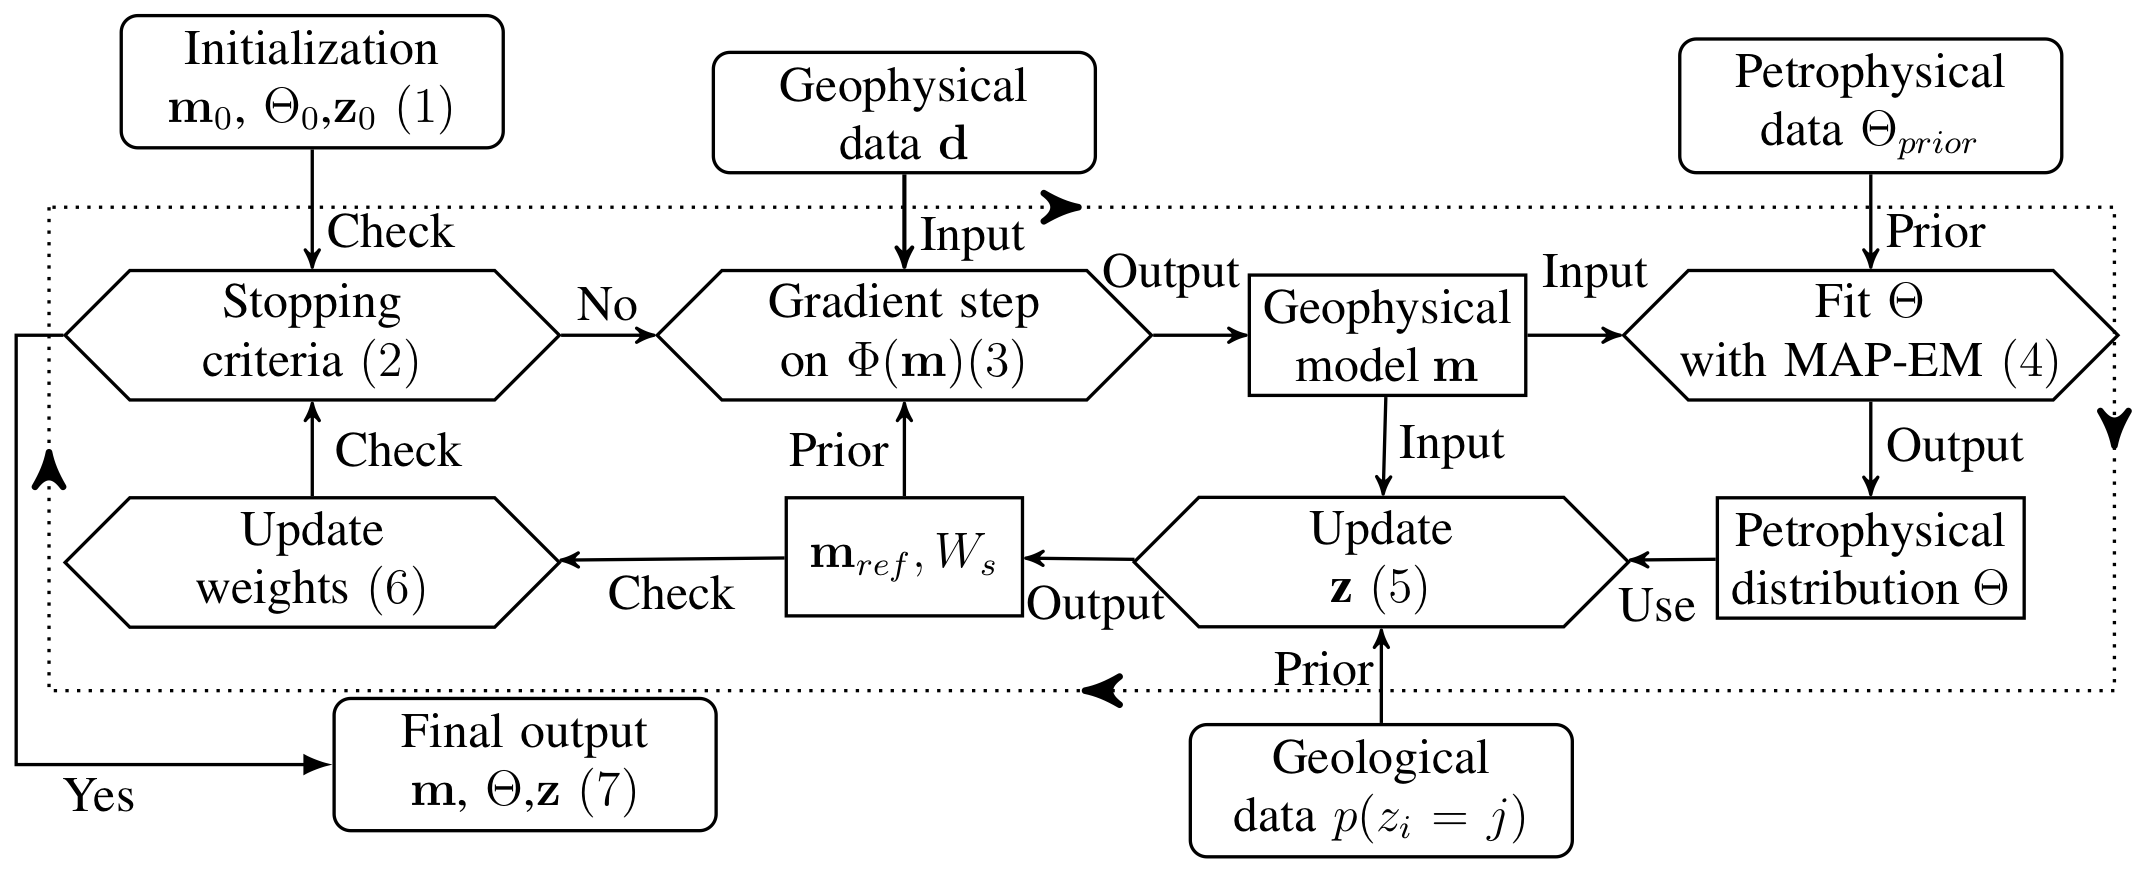
\includegraphics[width=\columnwidth]{./Fig/LowRes/Flowchart.png}
    \caption{A visual pseudocode of our iterative cyclic framework to include geological and petrophysical information into geophysical inversion. The numbers correspond to the steps displayed in algorithm 1.}
    \label{Flowchart}
\end{figure}
